%!TEX root = ../thesis.tex
%*******************************************************************************
%****************************** Second Chapter *********************************
%*******************************************************************************

\chapter{Computational methods \label{chap:2}}
%
\ifpdf
    \graphicspath{{Chapter2/Figs/Raster/}{Chapter2/Figs/PDF/}{Chapter2/Figs/}{Chapter2/Figs/Vector/}}
\else
    \graphicspath{{Chapter2/Figs/Vector/}{Chapter2/Figs/}}
\fi
%
Theories behind the calculations are the core component in the material properties determination process. Its correctness, accuracy and implementation directly influence the quality of its predictions. In this chapter, I will introduce relevant theoretical models, approximations and their implementations in commonly used software packages.
%
\section{Theory}
\subsection{Density Functional Theory}
%
Density functional theory (DFT) is one of the most widely used quantum mechanical methods to calculate the properties of materials. Its applicable length and time scales are in nanometre and picoseconds, respectively. These scales are longer than that for quantum Monte Carlo simulations but lower than that for semi- or full-empirical methods. This is also true in the accuracy verse size-of-the-system plot in \autoref{fig:dft_ac}. However, the accuracy of the different methods can be higher than what is shown in the figure, this is because a large part of the error can be attributed to the uncertainty of the experimental results that these methods are compared to\cite{Kirklin2015}. As I will discuss in the later section, if a DFT method is compared with a highly accurate theoretical benchmark method, DFT would have a precision around 1 meV/atom. Particularly, for bulk or nanostructures, DFT can be used to even quantitatively predict the properties of materials. Since DFT is based on Hohenberg-Kohn theorems\cite{Hohenberg1964} and Kohn-Sham equations\cite{Kohn1965}, here I will briefly give an overview of these two methods without putting too much stress on their derivations which have been extensively documented in textbooks. 
%
\begin{figure}[htbp!] 
\centering  
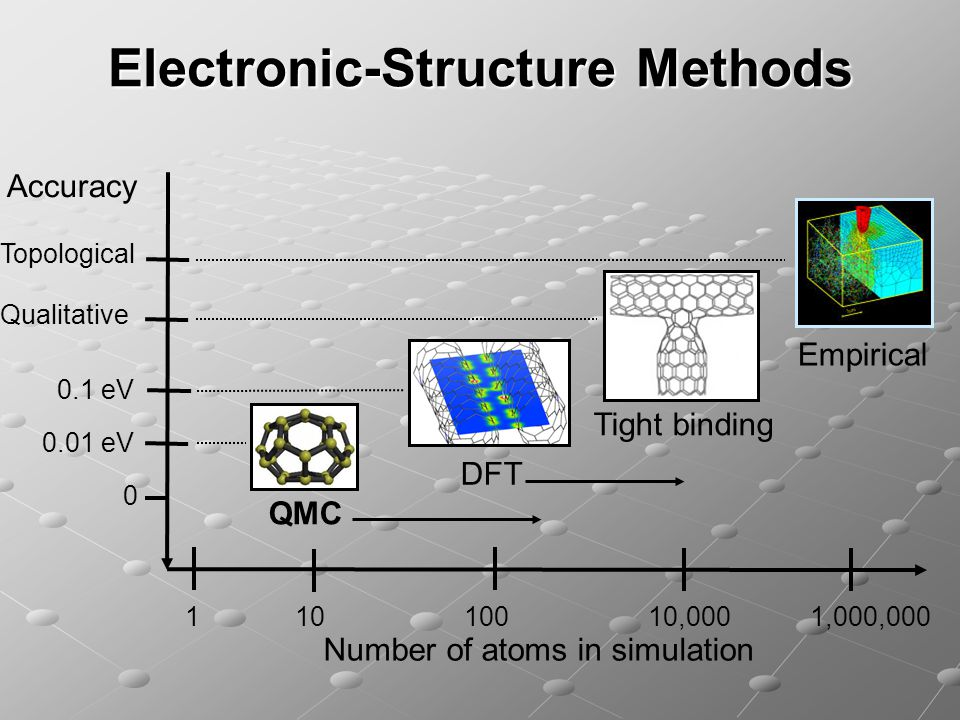
\includegraphics[width=0.9\textwidth]{dft1.jpg}
\caption[Comparison of different electronic structure calculation methods]{ Comparison of the accuracy and the size of different electronic structure calculation methods. Image source: Ref. \cite{dft_ac}}  
\label{fig:dft_ac}
\end{figure} 
%
Materials are made from atoms that contain electrons and nuclei. The type of the nuclei and the interactions between these give rise to various materials and their properties. The interactions are mainly electrostatic or Coulombic. While electrons must be described with quantum mechanics, the nuclei can be treated as classical particles. The equation governing the electron behaviour is the Schr\"{o}dinger equation. It can be written as follows:\footnote{Equations in this chapter are written in cgs form: length, mass, time and energy are in the units of centimetre, gram, second and erg, respectively. Additionally, fundamental constants $\hbar$, $e^2$ and $m$ are set to unity.}
\begin{equation}\begin{aligned}
\hat{H}\mathit{\Psi}_\alpha &(\vec{r_1}\sigma_1,\ldots,\vec{r_N}\sigma_N) \\
&=\left[ -\frac{1}{2}\sum^N_{i=1}\nabla_i^2+\sum^N_{i=1}\upsilon(\vec{r}_i)+\frac{1}{2}\sum_{i=1}\sum_{j\neq i}\frac{1}{|\vec{r}_i-\vec{r}_j|}\right]\mathit{\Psi}_\alpha(\vec{r_1}\sigma_1,\ldots,\vec{r_N}\sigma_N)  \\
&=\left( \hat{T} + \hat{V}_{ext} + \hat{V}_{ee}\right)\mathit{\Psi}_\alpha(\vec{r_1}\sigma_1,\ldots,\vec{r_N}\sigma_N) \\
&=E_\alpha\mathit{\Psi}_\alpha(\vec{r_1}\sigma_1,\ldots,\vec{r_N}\sigma_N) .
\end{aligned}\end{equation}
In the above equation, $\hat{H}$ is the total Hamiltonian, $\hat{T}$ is the kinetic energy, $\hat{V}_{ext}$ is the interaction between electrons and nuclei. Here we already started with the first approximation: Born–Oppenheimer approximation\cite{Born1927}. This approximation neglects the dynamics of nuclei, thus electrons are considered moving in a static potential generated by their interaction with all nuclei. $\hat{V}_{ee}$ is the interaction between electrons. The first two terms sum over all $N$-electrons, and the last one sums over all pairs of $N$-electrons. $\vec{r}$ is the electron position, $\sigma$ is the z-component of the electron spin (+$\frac{1}{2}$,-$\frac{1}{2}$). $\mathit{\Psi}$ is the $N$-electron wave function, which should be antisymmetric under the interchange of the orbital and the spin coordinates of two electrons (i.e. fermionic character for electrons) and it should also satisfy the boundary condition of the system (e.g. quantum confinement in a low-dimensional system). $E$ is the total energy, and $\alpha$ is the complete set of $N$-electron quantum numbers. 

Following the constrained search algorithm introduced by M. Levy\cite{Levy1979}, the ground-state energy $E$ can be found by minimizing the expectation value of the total Hamiltonian with respect to the wave function:
\begin{equation}
E=\min_\mathit{\Psi}\bra{\mathit{\Psi}}\hat{H}\ket{\mathit{\Psi}}.
\end{equation}
Here we take two steps for the minimization. For the first step, we minimize with respect to all wave functions that give the same density $n(\vec{r})$:
\begin{equation}
E=\min_{\mathit{\Psi}\rightarrow n}\bra{\mathit{\Psi}}\hat{T}+\hat{V}_{ee}\ket{\mathit{\Psi}}+\int dr^3\upsilon(\vec{r})n(\vec{r}).
\end{equation}
Then with the resulting wave function $\mathit{\Psi}^{min}_n$ that yields the minimum energy $E$ and is associated with the density $n(\vec{r})$, we can construct the universal functional $F[n(\vec{r})]$:
\begin{equation}
\min_{\mathit{\Psi}\rightarrow n}\bra{\mathit{\Psi}}\hat{T}+\hat{V}_{ee}\ket{\mathit{\Psi}}=\bra{\mathit{\Psi}^{min}_n}\hat{T}+\hat{V}_{ee}\ket{\mathit{\Psi}^{min}_n}=F[n(\vec{r})].
\end{equation}
As can be seen in this equation, a functional is a function of a function. For the second step, we minimize with respect to all densities $n(\vec{r})$:
\begin{equation}
E=\min_n \left\lbrace F[n(\vec{r})] + \int dr^3\upsilon(\vec{r})n(\vec{r}) \right\rbrace,
\end{equation}
where $\upsilon(\vec{r})$ is kept fixed during the minimization. The resulting density is the ground-state density that gives the lowest ground state energy. This is known as the density variational principle, which is also the main idea of the Hohenberg-Kohn theorems. For the completeness, the theorems are present in the following:
\begin{theorem}
The external potential, $V_{ext}(\vec{r})$, of any system of interacting particles is uniquely determined (up to a constant) by the particle density, $n_0(\vec{r})$, of the ground state.
\end{theorem}
\begin{theorem}
The ground state energy of a system with an external potential $V_{ext}(\vec{r})$ is given by the minimum value of the energy functional $E_{HK} [n]$ and the density for which this minimum is reached corresponds with the ground state density $n_0(\vec{r})$.
\end{theorem}
Now, the main problem is to find an approximated expression of $F[n(\vec{r})]$. Kohn-Sham equation is a elegant way to do this. It aims to construct a non-interacting system where kinetic energy can be calculated exactly, then add a local external potential $V_{KS}(\vec{r})$. The $F[n]$ decomposes into the following, where $E_{XC}[n]$ is the exchange-correlation (XC) energy:
\begin{equation}
F[n]=T_s[n]+E_H[n]+E_{XC}[n],
\end{equation}
where $T_s[n]$ is the non-interacting kinetic energy functional, and $E_H[n]$ is the Hartree energy functional:
\begin{equation}
E_H[n]=\frac{1}{2}\int d^3r\int d^3r\prime\frac{n(\vec{r})n(\vec{r\prime})}{|\vec{r}-\vec{r\prime}|}.
\end{equation}
Apart from the last term, $E_{XC}[n]$, everything else can be exactly calculated for a non-interacting system for given density. By imposing a normalisation constraint on the electron density, $\int n(\vec{r})d\vec{r}=N$, we have
\begin{equation}
\frac{\delta F[n]}{\delta n(\vec{r})}=-\upsilon(\vec{r}).
\end{equation}
Therefore, the effective local potential $V_{KS}(\vec{r})$ will be
\begin{equation}
V_{KS}(\vec{r})=\upsilon(\vec{r})+\frac{\delta E_H[n]}{\delta n(\vec{r})}+\frac{\delta E_{XC}[n]}{\delta n(\vec{r})},
\end{equation}
and the Kohn-Sham equation reads
\begin{equation}\label{eq:1}
\left[ -\frac{1}{2}\nabla_i^2+\upsilon(\vec{r})+\frac{\delta E_H[n]}{\delta n(\vec{r})}+\frac{\delta E_{XC}[n]}{\delta n(\vec{r})}\right]\mathit{\psi}_\alpha(\vec{r}\sigma)=\varepsilon_\alpha\mathit{\psi}_\alpha(\vec{r}\sigma),
\end{equation}
and ground-state density is 
\begin{equation}\label{eq:2}
n(\vec{r})=\sum_\alpha^{occ.}\sum_\sigma|\mathit{\psi}_\alpha(\vec{r}\sigma)|^2.
\end{equation}
This can be solved self-consistently. An initial guess of the density $n(\vec{r})$ determines the effective potential $V_{KS}(\vec{r})$, then the wave functions $\mathit{\psi}_\alpha(\vec{r}\sigma)$ can be calculated from \autoref{eq:1}, a new density is calculated through \autoref{eq:2}. This procedure is repeated until self-consistency is reached. 
\subsection{Exchange-correlation functional}
The XC energy functional is not known exactly and therefore needs to be approximated. The choice of it directly influences the accuracy of the results. This is because, although it is often a small fraction of the total energy, its contribution to the chemical bonding and the formation energy is relatively important. For the XC approximation, the generalized gradient approximation (GGA) has become popular in solid state calculations. It is a further upgrade of its previous version, the local density approximation (LDA). The LDA has the following form:
\begin{equation}
E_{XC}^{LDA}[n]=\int n(\vec{r})\epsilon_{XC}[n(\vec{r})]d\vec{r}.
\end{equation}
$\epsilon_{XC}[n(\vec{r})]$ is the XC energy for an homogeneous electron gas having density $n$, and it is usually taken from quantum Monte Carlo calculations. Whereas the GGA further includes the derivative of density, $\nabla n(\vec{r})$, as an argument for $\epsilon_{XC}$, thus it reads
\begin{equation}
E_{XC}^{GGA}[n]=\int \epsilon_{XC}[n(\vec{r}),\nabla n(\vec{r})]d\vec{r}.
\end{equation}
In contrast to LDA, there is no unique input for $\epsilon_{XC}[n(\vec{r}),\nabla n(\vec{r})]$. Different constructions for GGA usually named with the corresponding authors, e.g. PW91-GGA stands for Perdew and Wang's GGA construction in 1991\cite{Perdew1991,Perdew1992} and PBE-GGA stands for \citet{GGA-PBE2}'s construction. They are the most popular GGA approximations for solid state systems. 
\subsubsection{Jacob's ladder}
Jacob's ladder is a ladder connecting earth and heaven that biblical Patriarch Jacob dreamed about. Professor John P. Perdew, who is known for profound contribution to DFT and XC functionals, used it analogously to describe the hierarchy of density functional approximations in terms of their accuracies, see \autoref{fig:dft_jl}.  
\begin{figure}[htbp!] 
\centering  
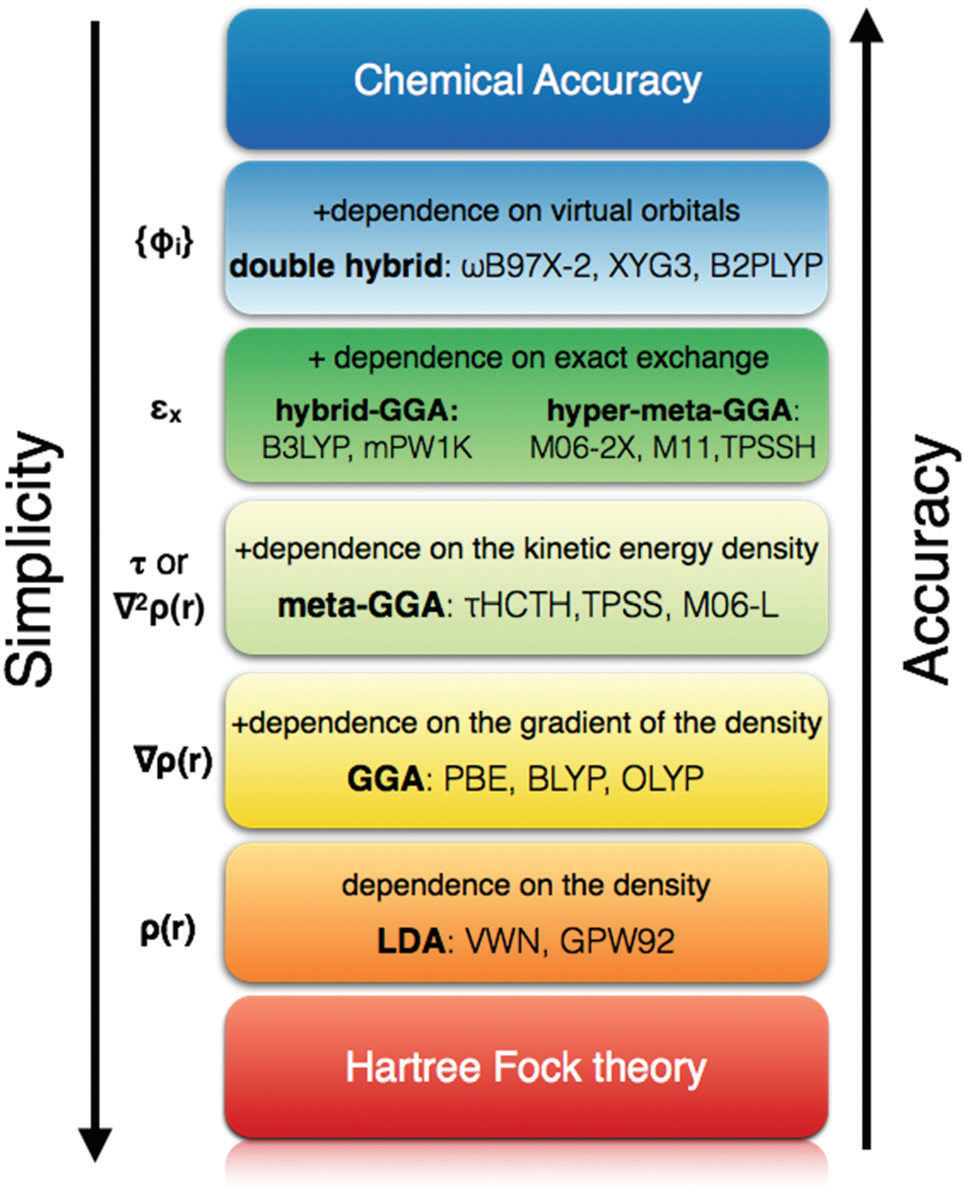
\includegraphics[width=0.7\textwidth]{jacobs.png}
\caption[Jacob's ladder for DFT approximations]{ Jacob's ladder for DFT approximations. Image source: Ref. \cite{Peng2016}}  
\label{fig:dft_jl}
\end{figure} 
Each rung is a level of approximation constructed with different formalisms. From LDA and GGA as mentioned before to meta-GGA which includes the Kohn-Sham kinetic energy density. Next method higher in the ladder is the hybrid functionals which incorporates a part of the exact exchange from Hatree-Fock (HF) theory. For example, the PBE0 functional\cite{Carlo1999} has the following definition:
\begin{equation}
E_{XC}^{PBE0}=\frac{1}{4}E_X^{HF}+\frac{3}{4}E_X^{PBE}+E_C^{PBE},
\end{equation}
and the HSE06 (Heyd-Scuseria-Ernzerhof)\cite{Jochen2003} takes into account the screened Coulomb potential for the exact part:
\begin{equation}
E_{XC}^{HSE}=\beta E_X^{HF,SR}(\omega)+(1-beta)E_X^{PBE,SR}(\omega)+E_X^{PBE,LR}(\omega)+E_C^{PBE},
\end{equation}
where $\beta$ is the mixing parameter and $\omega$ is the parameter to control the screening range which defines the short-range, SR, and long-range, LR, parts. The values of $\beta=1/4$ and $\omega=0.2$ corresponding to HSE06 functional which gives accurate band gaps and lattice constants, see the mean absolute error (MAE) of different functionals in \autoref{fig:dft_ex}. 
\begin{figure}[htbp!] 
\centering  
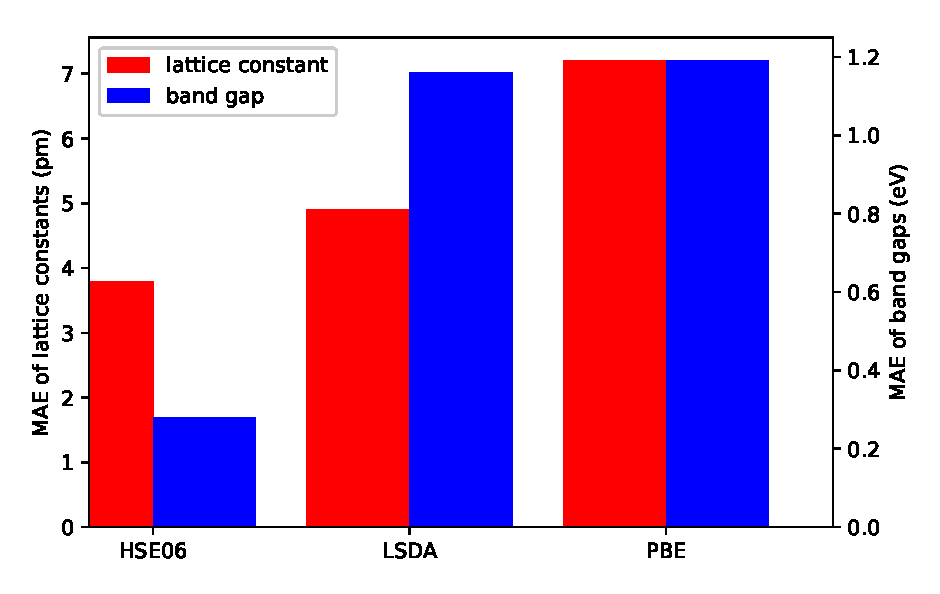
\includegraphics[width=0.9\textwidth]{lat_ex.eps}
\caption[MAE of the equilibrium lattice constants and band gaps of different functionals]{ MAE of the equilibrium lattice constants and band gaps of different functionals on SC40 solid test set\protect\footnotemark[1]. Data source: \cite{Lucero2012}}  
\label{fig:dft_ex}
\end{figure} 
The highest ranked funcional is the double hybrid which includes the unoccupied orbitals as well, e.g. Random Phase Approximation\cite{Langreth1980}. 
\footnotetext[1]{The SC40 test set is a collections of 40 elementary and binary solid compounds of various structures with a wide range of band gaps}
\subsubsection{Band gap problem}
As shown in \autoref{fig:dft_ex}, band gap estimated in LDA and GGA is quite poor. This can be attributed to the highly non-analytical and non-local behaviours of the XC energy functional. To understand this, let's look at the definition of the band gap $E_{g}$:
\begin{equation}
E_{g}=I-A=\varepsilon_{N+1}^{KS,HOMO}-\varepsilon_N^{KS,HOMO},
\end{equation}
where $I$ is the ionization energy, which is the energy change by removing one valence electron. $A$ is the electron affinity, which is the energy change by adding one electron to a neutral system. $\varepsilon_N^{KS}$ is the Kohn-Sham orbital energy for N-electron system. $HOMO$ and $LUMO$ stand for the highest and the lowest occupied molecular orbital, respectively. For a non-interacting Kohn-Sham system, $E_{g}^{KS}$ can be calculated as follows:
\begin{equation}
E_{g}^{KS}=\varepsilon_{N}^{KS,LUMO}-\varepsilon_{N}^{KS,HOMO}.
\end{equation}
This leads to 
\begin{equation}
E_{g}=E_{g}^{KS}+\Delta_{XC},
\end{equation}
where $\Delta_{XC}$ is the orbital shift caused by adding an extra electron: $\varepsilon_{N+1}^{KS,HOMO}-\varepsilon_{N}^{KS,LUMO}$.
\begin{figure}[htbp!] 
\centering  
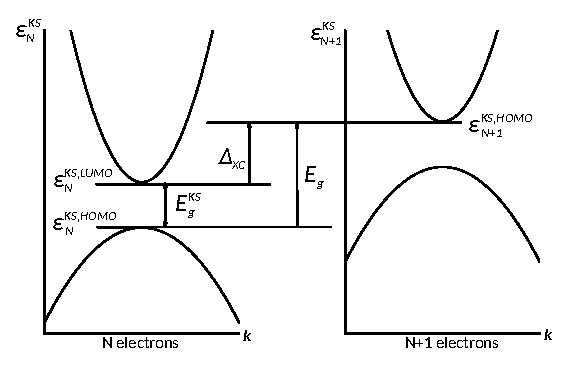
\includegraphics[width=0.9\textwidth]{Eg.eps}
\caption[Schematic illustration of the relation between $E_g$ and $E^{KS}_g$]{ Schematic illustration of the relation between $E_g$ and $E^{KS}_g$. Image is adapted from Ref. \cite{fiolhais2008primer}.}  
\label{fig:dft_eg}
\end{figure} 
The $\Delta_{XC}$ exclusively depends on the non-analyticity of the XC potential $\frac{\delta E_{XC}[n]}{\delta n(\vec{r})}$, since the Hartree potential explicitly depends on the density. In other words, it means the energy increase by adding an extra electron in the extended system is of the order of 1 eV, even though, it is an infinitesimal density change. If the XC energy functional were analytic, the infinitesimal density variation would not introduce a large potential change, hence $\Delta_{XC}$ is small or equals to zero, and $E_g \approx E^{KS}_g$. The accuracy of the band gap, when compared to experiment measurement, would be only limited by the error that is inherent to different functionals. However, $\Delta_{XC}$ usually is not zero and it is responsible for the 80\% of the LDA band gap error\cite{Godby1988}. 
\section{Implementation}
The implementations of the theory in the last section are crucial and not always straightforward. Many of the quantities are represented with technically easy-implemented functions, and they have to be finite in size or quantity. A question will rise on how large the size or the resolution has to be. This is equivalent to the computational convergence. Here we review two of the most important convergence parameters: $\mathbf{k}$ points and cut-off energy of the basis set.
\subsubsection{k points}
According to Bloch's theorem, the solution of the Schr\"{o}dinger equation for a periodic system, e.g. a crystal with a well-defined unit cell, can be expressed through the following:
\begin{equation}\label{imp:bloch}
\phi_{\mathbf{k}}(\mathbf{r})=e^{i\mathbf{k}\cdot\mathbf{r}}u_{\mathbf{k}}(\mathbf{r}),
\end{equation}
where $\phi$ is the wave function, $u$ is a function having the same periodicity as the crystal. The vector $\mathbf{r}$ and $\mathbf{k}$ are associated with the real and the reciprocal space ($\mathbf{k}$ space), respectively. Particularly, each point in $\mathbf{k}$ space is associated with a unique $\mathbf{k}$ vector and is usually called a $\mathbf{k}$ point. Making use of the symmetry of the system, all inequivalent $\mathbf{k}$ points are contained inside a finite subspace of $\mathbf{k}$ space, called the first Brillouin zone (FBZ). Quantity evaluations are mostly done through the integration of wave functions, or other functions having $\mathbf{k}$ dependence, over the FBZ. This integration has to be done numerically since the explicit relation of $\phi$ and $\mathbf{k}$ is unknown. In practice, the FBZ is discretized into a grid defined by the mesh of the k-points. This mesh has to be large enough for the accurate sampling of FBZ, yet it should be small enough to reduce the computational time and resource. This is one of the convergence tests that need to be done in order to obtain reliable results. Usually, metals need more k-points than semiconductors. This is because the highest occupied valence band crosses the Fermi energy in metals, hence the integration for all occupied states is done for a discontinuous function that excludes unoccupied states.  Whereas for a semiconductor or insulator, the highest occupied valence band is completely occupied, therefore the integration is for a continuous function. Smearing is one of the ways to transform a discontinuous function in metal into a continuous one by smearing out the edge using a smearing function, such as Fermi-Dirac function. The range of smearing has to compromise between the computation efficiency and correctness: Too large will give wrong integration results of the total energy, while too small become useless therefore one again needs more k-points.
\subsubsection{Basis set, cut-off energy }
Now let us look back at \autoref{imp:bloch}. There we can identify $e^{i\mathbf{k}\cdot\mathbf{r}}$ as a plane wave, $u_{\mathbf{k}}(\mathbf{r})$ is periodic in space and it can be expanded in terms of a set of plane waves as well:
\begin{equation}
u_{\mathbf{k}}(\mathbf{r})=\sum_{\mathbf{G}}c_{\mathbf{G}}e^{i\mathbf{G}\cdot\mathbf{r}},
\end{equation}
where $c_{\mathbf{G}}$ is the coefficient that determines the magnitude of the plane wave $e^{i\mathbf{G}\cdot\mathbf{r}}$. \autoref{imp:bloch} can now exclusively be represented with plane waves:
\begin{equation}
\phi_{\mathbf{k}}(\mathbf{r})=\sum_{\mathbf{G}}c_{\mathbf{k+G}}e^{i\mathbf{k+G}\cdot\mathbf{r}}.
\end{equation}
The summation in the above equation, for practical reasons, has to be truncated. The truncation is usually done for the kinetic energy:
\begin{equation}
E=\frac{1}{2}|\mathbf{k+G}|^2.
\end{equation}
The maximum kinetic energy, $E_{cut}$, is associated with a $\mathbf{G}$ vector and define the limit the summations. Here we arrived at another convergence parameter: the plane wave cut-off energy. Similar to the $\mathbf{k}$ points, it has to be large enough for the total energy to be converged in an acceptable precision range.  While too large will cost more computational resources without additional benefits.
\subsubsection{Pseudopotentials and projected augmented-wave method}
Considering the chemical inertness of the core electrons and their highly oscillating wave functions, their impact on the valence electrons is generally approximated by pseudopotentials in order to optimize the computational efficiency. It is a smooth function and has the ability to reconstruct the original core electron properties. Transferability of a pseudopotential is one of the most important factors that determine the performance of the potentials. In practice, a pseudopotential is usually constructed for one isolated atom of one element, while being used in complex multi-elements system, the potentials with higher transferability can simulate what a real atom will react to these different environments. Ultrasoft \cite{Ultrasoft1} and projected augmented-wave (PAW) \cite{PAW1,Kresse1999} are two types of the most popular pseudopotentials-based methods used in materials simulations. They are well-balanced between accuracy and computational cost. In this thesis, the PAW method is exclusively used for all calculations. This method combines the ideas of pseudopotentials method and all-electron methods. Same as in the case of pseudopotential, in PAW, the true wave function $\ket{\Psi_n}$ that are obtained from all-electron methods can be transformed into a smooth auxiliary function $\ket{\tilde{\Psi}_n}$ by a linear transformation operator $\mathcal{T}$. The partial waves $\ket{\phi_i}$ is the complete basis set that expands the wave function and it can be also related to auxiliary partial waves $\ket{\tilde{\phi}_i}$:
\begin{equation}
\ket{\phi_i}=\mathcal{T}\ket{\tilde{\phi}_i},
\end{equation}
where $i$ is a complete set of quantum numbers. The true and the auxiliary wave functions are identical outside the cur-off radius $r_c$:
\begin{equation}
\phi_i(\mathbf{r})=\tilde{\phi}_i(\mathbf{r})\text{, for }|\mathbf{r}-\mathbf{R}|>r_c,
\end{equation}
where $\mathbf{R}$ is the position of the atom. The transformation operator $\mathcal{T}$ takes the following form:
\begin{equation}
\mathcal{T}=1+\sum_i(\ket{\phi_i}-\ket{\tilde{\phi}_i})\bra{\tilde{p}_i},
\end{equation}
where $\tilde{p}_i$ is the projector functions that capture the character of true wave function within a radius of $r_c$. Now the all-electron wave functions can be reconstructed through the smooth auxiliary functions and projector functions :
\begin{equation}
\ket{\Psi_n}=\ket{\tilde{\Psi}_n}+\sum_i(\ket{\phi_i}-\ket{\tilde{\phi}_i})\braket{\tilde{p}_i|\tilde{\Psi}_n}.
\end{equation}
The PAW method expresses the true all-electron wave functions with smooth functions that can be easily implemented and perform more efficiently as compared to the all-electron wave functions, moreover the accuracy of the calculations are comparable to that for the all-electron ones.
\subsection{Software Packages}
There are more than 70 different software packages capable of performing density functional theory calculations according to Wikipedia\cite{dft_sws}. They mainly differ in the type of pseudopotentials if there is any, the type of basis set is used to expand the wave function, in which programming language it is written and whether or not it is free or commercial etc. \citet{Lejaeghereaad3000} have compared 40 different implementations and their accuracy by comparing their results to a highly accurate all-electron method. They concluded that all codes or methods yield generally consistent results. The accuracy of the codes which were developed in the recent years is higher than the earlier ones. The Vienna $Ab$ $initio$ Simulation Package (VASP) \cite{VASP1,VASP2} with its PAW method is one of the most accurate codes those are concluded from this study. Its well-optimized performance on supercomputers gives good results in less time as compared with the others. This code will be used as the main tool for all the calculations done in this thesis.